\chapter{Fundamentação Teórica}

Este capítulo detalha os principais conceitos e tecnologias aplicados no projeto: Internet das Coisas, sistemas distribuídos, protocolo HTTP, AOSP, desenvolvimento Android e ESP32 com NodeMCU. Portanto, 
a seguinte seção aborda como os conceitos citados contribuíram para o desenvolvimento deste trabalho de conclusão de curso, possibilitando
ao leitor uma visão geral das competências necessárias em sua execução. 

\section{Internet das Coisas}

O termo \textit{Internet das Coisas} (\textit{IoT}, da expressão em inglês \textit{Internet of Things}) foi utilizado primeiramente em 1999 pelo então pesquisador do \textit{Massachusetts Institute of Technology} (MIT) Kevin Asthon em uma apresentação na Procter \& Gamble (P\&G) sobre a tecnologia do \textit{Radio Frequency Identification} (RFID). O RFID é uma tecnologia utilizada para a identificação e rastreamento de objetos, animais ou pessoas através de ondas de rádio. Portanto, Asthon pontuou a possibilidade de utilizar tal ferramenta para gerenciar a cadeia de suprimentos da empresa, pois sua capacidade de ler vários emissores simultaneamente, sem a necessidade de linha de visão direta entre o leitor e a tag (ao contrário de códigos de barras) torna o controle mais preciso \cite{iot-first-definition}. 

\textit{IoT} possui muitas definições. Embora não haja um consenso convergente para uma definição única, podemos discutir sobre seu impacto na sociedade atual e aspectos importantes que toda solução na área possui. No livro \textit{The Internet  of Things}, escrito por Samuel Greengard, o tema é abordado como um eventos disruptivo, onde a linha que separa o humano e a tecnologia se torna cada vez menos visível, porém o texto aborda não somente a capacidade de conexão entre as máquinas, e sim a autonomia e "inteligência" cada vez maior dos sistemas embarcados \cite[pp. 17]{book-iot}. Essa visão de tecnologia integrada no cotidiano é o conceito que o autor Mark Weiser aborda no seu artigo denominadao \textit{The Computer for the 21st Century}. A computação úbiqua é o processo de tornar os computadores "invisíveis" aos nossos olhos, desenvolvendo a comunicação com tais ferramentas eletrônicas o mais próximo possível da forma humana, ou seja, o dispositivo tem conexão com a rede e responde aos estímulos do usuário por interfaces naturais, exemplo da fala e gestos com as mãos \cite{ubiquitous-computing}.

Portanto, o significado mais comum de \textit{IoT} talvez seja a de dispositivos eletrônicos conectados na internet, permitindo enviar e receber dados do ambiente real. No entanto, apenas conectar dispositivos não é uma solução em Internet das Coisas, pois essa área envolve o uso de protocolos de comunicação, eletrônica de baixo consumo energético, plataformas em nuvens e outras inúmeras áreas do conhecimento. Os dados coletados de sensores atuam como combustível para a execução de um fluxo de tomada de decisão \cite{iot-cycle}. 

\begin{figure}[ht]
    \centering
    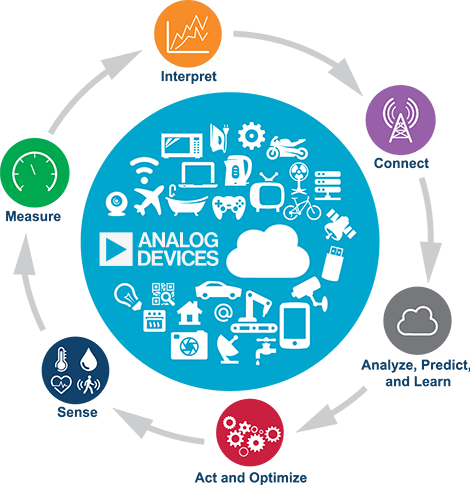
\includegraphics[width=.50\textwidth]{img/iot-cycle.png}
    \caption{Ciclo de IoT. Fonte:\cite{iot-cycle}}\label{figIoTCycle}
\end{figure}

Atualmente, a coleta de dados e uso de ferramentas de análise são o principal recursos de empresas competitivas no gerenciamento de suas atividades. Com o avanço da área de telecomunicações, as organizações têm potencial de transformar grandes volumes de dados em \textit{insights} poderosos, que orientam a tomada de decisões da equipe de gestão. Portanto, a Internet das Coisas representa uma tendência forte e disruptiva na sociedade.

\section{Sistemas Distribuídos}

``Um sistema distribuído é aquele no qual os componentes localizados em computadores interligados em rede se comunicam e coordenam suas ações apenas passando mensagens.'' \cite[pp. 1]{sistemas-distribuidos-coulouris2013}.
A definição apresentada pelo autor leva em conta dois importantes fatores: o primeiro é representado pela comunicação via rede de computadores, e o segundo está relacionado ao provisionamento de um serviço.
O mundo atual oferece inúmeros exemplos da importância dos sistemas distribuídos no desenvolvimento socieconômico: a modalidade de educação a distância \cite{mec-ead}, no qual serviços web e compartilhamento
multimídia são responsáveis por possibilitar o acesso ao ensino de qualidade ao público distante fisicamente dos grandes centros de ensinos, como, por exemplo, cidades do interior ou comunidades ribeirinhas; o comércio digital, cujo crescimento do \textit{e-Commerce},
resultou em um faturamento superior à R\$ 180 billhões de reais em 2023 no Brasil, de acordo com dados da Associação Brasileira de Comércio Eletrônico \cite{abcomm-ecomerce}; e transações distribuídas, porém auditáveis e transparentes, em redes \textit{blockchain} descentralizadas \cite{juliana-blockchain}, sendo sua 
aplicação mais conhecida as criptomoedas, pois a tecnologia permite a transferência de recursos e o armazenamento de todas as operações.  

Portanto, o sistema distribuído tem foco no compartilhamento de recursos. Em relação a sua implementação, o comportamento mais comum visto na web é o modelo cliente/servidor, pois 
grande das aplicações na web são construídos na sua premissa, por exemplo serviço de e-mail e sites. 
A nível de Sistema Operacional, o intuito da comunicação entre os processos executados em computadores hospedeiros interlidados em rede é o gerenciamento e acesso de recursos, portanto um cliente realiza
uma solicitação ou chamada ao servidor, que por sua vez executa uma tarefa interna para o processamento de toda a chamada e gera um resultado para o cliente em espera, ou em outras palavras, faz a comunicação do tipo requisição/resposta \cite[pp. 16]{sistemas-distribuidos-coulouris2013}. 

\section{Protocolo HTTP}

O HTPP (do inglês \textit{HyperText Transfer Protocol})

\section{AOSP}

AOSP é coisa e tal

\section{Desenvolvimento Android}

Android é coisa e tal 

\section{ESP32 e NodeMCU}